\documentclass[a4paper,12pt]{book}
\usepackage[spanish]{babel}
\usepackage[latin1]{inputenc} 
\usepackage{makeidx}
\usepackage[dvipsnames,svgnames,table]{xcolor}
\usepackage[export]{adjustbox}
\usepackage{graphicx}
\usepackage{ulem}
\usepackage[hidelinks]{hyperref} 
\usepackage{amsmath}
\usepackage{amsthm}
\usepackage{amssymb}
\usepackage[paperwidth=595pt,paperheight=841pt,top=56pt,right=86pt,bottom=84pt,left=71pt]{geometry}
\usepackage{setspace}
\usepackage{float}
\usepackage{subfiles}
\usepackage[final]{pdfpages}
\usepackage{fancyhdr}
\usepackage[figuresright]{rotating}
\usepackage{caption}
\usepackage{verbatimbox}

\title{Titulo}

% sangr�a y separacion entre parrafos
\setlength{\parindent}{0pt}

\makeatletter
\renewcommand\chapter{\if@openright\cleardoublepage\else\clearpage\fi
                    \thispagestyle{empty}%
                    \global\@topnum\z@
                    \@afterindentfalse
                    \secdef\@chapter\@schapter}
\makeatother
	\onehalfspacing
	\pagestyle{plain}
	
\newtheorem{theorem}{Teorema}[section]
\newtheorem{lemma}[theorem]{Lema}
\newcommand{\definition}{\textbf{Definici�n}}
\newcommand{\bmathcal}{\mathcal{B}}
\newcommand{\dmathcal}{\mathcal{D}}
\newcommand{\vmathcal}{\mathcal{V}}
\newcommand{\ESPACIO}{\hspace{.25in}}
\newcommand{\IF}{\textbf{if }}
\newcommand{\THEN}{\textbf{then }}
\newcommand{\ELSE}{\textbf{else }}
\newcommand{\REPEAT}{\textbf{repeat }}
\newcommand{\UNTIL}{\textbf{until }}
\newcommand{\FOREACH}{\textbf{foreach }}
\newcommand{\DO}{\textbf{do }}
\newcommand{\RETURN}{\textbf{return }}
\renewcommand\qedsymbol{QED}

\makeindex


\begin{document}

	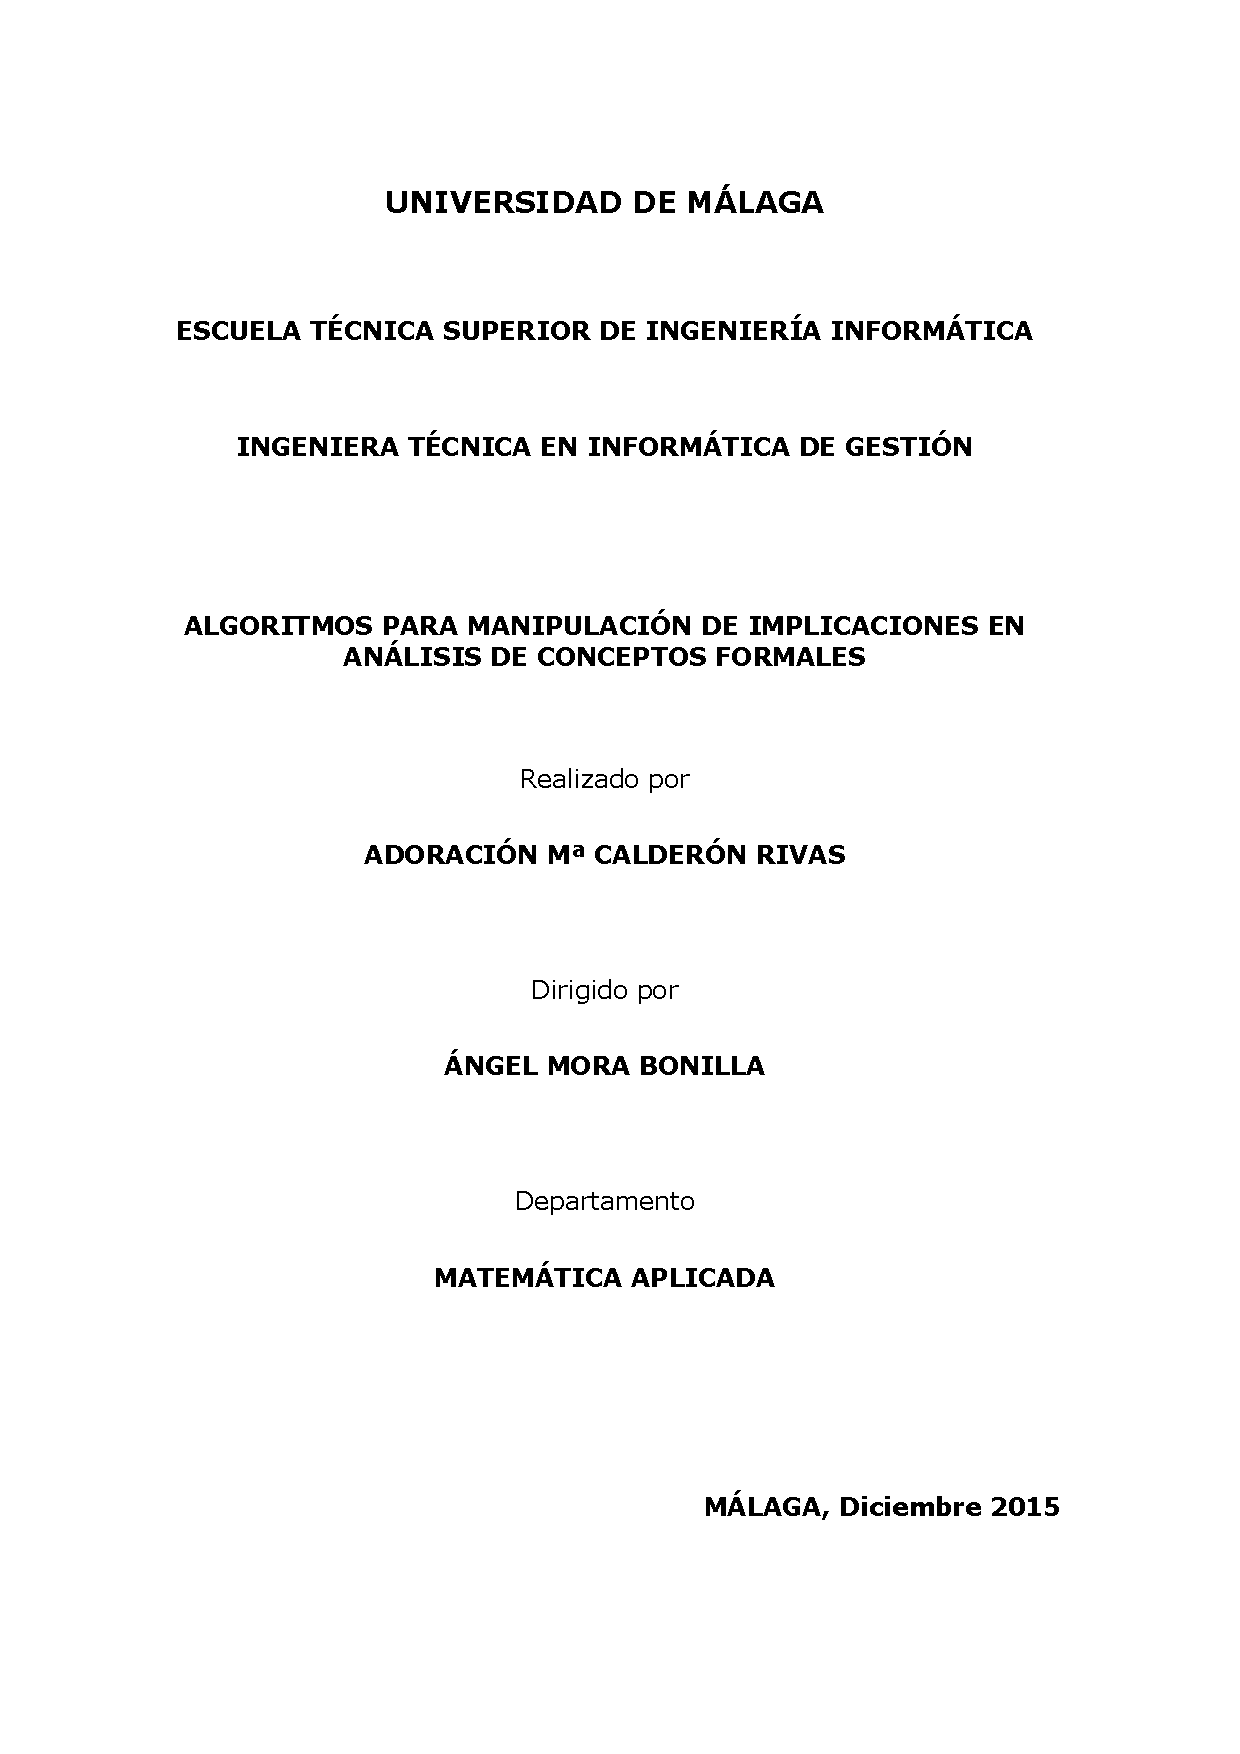
\includepdf[pages=-]{ext/paginas_iniciales.pdf}	
	
	% quitar la numeraci�n de p�ginas
	\cleardoublepage
	\pagenumbering{gobble}

	\tableofcontents
	
	% a�dir la numeraci�n de p�ginas
	\cleardoublepage
	\pagenumbering{arabic}

	\subfile{tex/introduccion.tex}
	
	\subfile{tex/acf.tex}
		
	\subfile{tex/algoritmos_bases.tex}
		
	\subfile{tex/herramienta_impl.tex}
			
	\subfile{tex/comparativa_algoritmos.tex}
	
	\subfile{tex/analisis_aplicacion.tex}
		
	\subfile{tex/conclusiones.tex}
		

%------------------------- BIBLIOGRAFIA -------------------------------------------
\begin{thebibliography}{99}
	\bibitem{bib:ref1}
	E. Rodr�guez, K. Bertet, P. Cordero, M. Enciso, A. Mora y M. Ojeda-Aciego: {\it A method to build the Direct-Optimal Basis from
	an implicational system}.
	
	\bibitem{bib:ref2} K. V. Adaricheva and J. B. Nation and R. Rand, Ordered direct implicational basis of a finite closure
	system, International Symposium on Artificial Intelligence and Mathematics, ISAIM 2012.

	\bibitem{bib:ref3} K. Bertet, M. Nebut, Efficient algorithms on the Moore family associated to an implicational system, DMTCS,
	6(2): 315-338, 2004.

	\bibitem{bib:ref4} K. Bertet, B. Monjardet, The multiple facets of the canonical direct unit implicational basis, Theor.
	Comput. Sci., 411(22-24): 2155-2166, 2010.

	\bibitem{bib:ref5} K. Bertet, Some Algorithmical Aspects Using the Canonical Direct Implicationnal Basis, CLA:101-114, 2006.

	\bibitem{bib:ref6} K. Bertet, C. Demko, J.F. Viaud, C. Gu�rin, java-lattices: a Java for lattices computation,
	\url{http://thegalactic.org}, 2014.

	\bibitem{bib:ref7} P Cordero, A. Mora, M. Enciso, I.P�rez de Guzm�n, SLFD Logic: Elimination of Data Redundancy in Knowledge
	Representation, Lecture Notes in Computer Science, 2527: 141-150, 2002.

	\bibitem{bib:ref8} A. Mora, M. Enciso, P. Cordero, and I. Fortes, Closure via functional dependence simplification, I. J.of
	Computer Mathematics, 89(4): 510-526, 2012.

	\bibitem{bib:ref9} E. Rodr�guez Lorenzo, K. Bertet, P. Cordero, M. Enciso, A. Mora,  Direct-optimal Basis via Reductions, CLA:
	145-156, 2014.

	\bibitem{bib:ref10} E. Rodr�guez Lorenzo, K. Bertet, P. Cordero, M. Enciso, A. Mora, Ojeda-Aciego From Implicational Systems to
	Direct-Optimal bases: A logic-based Approach, Applied Mathematics \& Information Sciences, 2L: 305-317, 2015.
	
	\bibitem{bib:ref11} A. Mora, M. Enciso, P. Cordero, and I. P�rez de Guzm�n,Preprocessing Transformation for Functional
	Dependencies Sets Based on the Substitution Paradigm, Lecture Notes in Computer Science, 3040: 136-146, 2004.
	
	\bibitem{bib:ref12} Bertet, Karell and Demko, Christophe and Viaud, Jean-Fran�ois and Gu�rin, Cl�ment, {java-lattices}: a Java library for lattices computation, 	
			\url{http://thegalactic.github.io/java-lattices/, 2014}

	\bibitem{bib:ref13} Oracle, Java Platform, Standard Edition (Java SE) 8, \url{http://docs.oracle.com/javase/8/}
	
	\bibitem{bib:ref14} Oracle, JavaFX 2 Documentation, \url{http://docs.oracle.com/javafx/2/}
	
	\bibitem{bib:ref15} Oracle, Trail: Java Architecture for XML Binding, \url{https://docs.oracle.com/javase/tutorial/jaxb/}
	
	\bibitem{bib:ref16} QOS.ch, Simple Logging Facade for Java (SLF4J), \url{http://www.slf4j.org}
	
	\bibitem{bib:ref17} The Apache Software Foundation, Apache Commons CSV, \url{https://commons.apache.org/proper/commons-csv/} 
	
	\bibitem{bib:ref18} Google, Guava, Wiki \url{https://github.com/google/guava/wiki}
	
	\bibitem{bib:ref19} The Apache Software Foundation, Apache Maven Project, \url{https://maven.apache.org/}

	\bibitem{bif:ref20}  Object Management Group (OMG), Unified Modeling Language (UML) Resource Page, \url{http://www.uml.org/}
	
\end{thebibliography}
		
\end{document}